\section{Evaluation}
\label{sec:eval}
%This section presents the experimental results for Ostrich on an Intel 32-cores multicore machine. 
%In this section, we measured the performance and scalability of \myds, and compare it with Phoenix.  
We evaluate \myds and Phoenix on a 32-core Intel 4× Xeon E7-4820 system equipped with 128GB of RAM. 
The operating system is Ubuntu 12.04 with kernel 3.2.0 and glibc-2.15.
Benchmarks were built as 64-bit executables with gcc -O3.
We logically disable CPU cores using Linux’s CPU hotplug mechanism, which allows to disable or enable individual CPU cores by writing “0” (or “1”) to a special pseudo file (/sys/devices/system/cpu/cpuN/online), and the total number of threads was matched to the number of CPU cores enabled.
Each workload is executed 10 times. 
To reduce the effect of outliers, the lowest and the highest runtimes for each workload are discarded, and thus each result is the average of the remaining 8 runs.


%\subsection{ Performance Improvements Summary}
%\subsection{Benckmarks}
%The benchmark applications are derived from those
%supplied by Phoenix, and summarized in Figure 6. For
%StringMatch, LinearRegression and Histogram, the num-
%ber of keys is fixed and the number of pairs per key de-
%pends on the number of map input splits. The results for
%sections other than 5.4 use the workloads described in
%Figure 7. These are chosen to ensure the applications run
%for a moderately long time, but still fit in memory. The
%inputs are in the in-memory buffer cache.

Five MapReduce applications is used in the evaluation, including histogram (\codet{hist}), linear\_regression (\codet{lr}), string\_match (\codet{sm}), wordcount (\codet{wc}), and pca (\codet{pca}).
we report results using the large data sets available, which are summarized in Table \ref{}.

%These applications represent two different classes:


\subsection{Performance and Scalability}
Since there are many heap objects shared among threads in Phoenix, it is sensitive to memory allocator\cite{yoo2009phoenix2}.
The memory allocator in glibc (i.e. ptmalloc\cite{gloger1997ptmalloc}) does not scale on multicore system, while jemalloc\cite{evans2006jemalloc} can provide improved performance and scalability. 
Therefore, in this section, we first evaluate the scalability of Phoenix built with jemalloc, denoted as \codet{Phoenix-jemalloc}.
Then we measure the performance and scalability of \myds compared with \codet{Phoenix-jemalloc}.


%Therefore, in this section, we will evaluate performance and scalability of Phoenix built with both jemalloc and ptmalloc, denoted as \codet{Phoenix-jemalloc} and \codet{Phoenix-ptmalloc}, respectively.

%Phoenix-jemalloc版本scalability存在的问题
%Since Phoenix is sensitive to memory allocator\cite{yoo2009phoenix2}, in this subsection, 
%====================================================
%\subsubsection{Scalability of Phoenix}
%%We first evaluate the scalability of Phoenix built with jemalloc, a good scalable memory allocator, and than we measure the scalability of \myds to demonstrate the effectivity of \myds.
%
%\begin{figure}[!h!t]  
%	\centering
%	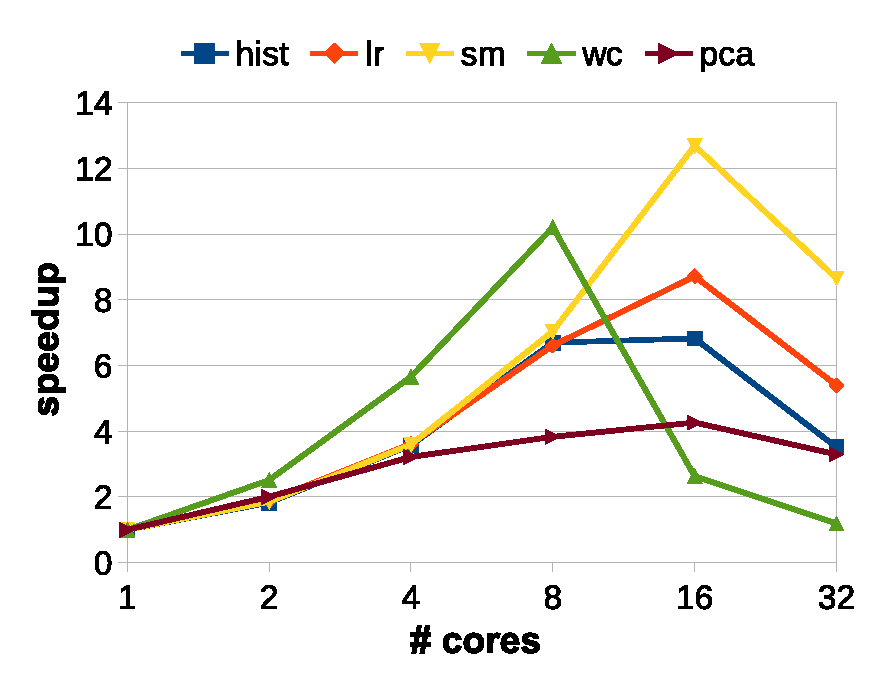
\includegraphics[width=0.45\textwidth]{eps/phoenix_speedup_jemalloc.eps}
%	\caption{speedup of Phoenix-jemalloc}
%	\label{fig:phoenix:speedup:jemalloc}
%\end{figure}
%
%%For linear\_regression (lr) and string\_match (sm),  using 16 or more  cores leads to speedup degradation.
%
%Figure \ref{fig:phoenix:speedup:jemalloc} illustrates the speedup of Phoenix built with jemalloc.
%We observe that applications scale well when the core count increases from 1 to 8.
%However, when the core count increases from 8 to 16 to 32, the speedup sharply degrades for \codet{wc} and from 16 to 32 cores for the other applications.
%%Phoenix performs well with less cores, it can not scale up 16 cores for all applications. 
%%Actually, when cores number exceed 8, the speedup of \codet{wc} and \codet{hist} on Phoenix begin degrading. 
%
%%Phoenix performs well with no more than 16 cores.
%%However, when core number exceed 16, .
%%For lr and sm, the speedup is degraded when cores is greater than 16.
%
%
%%on \codet{hist}, \codet{wc} and \codet{pca} when the number of core is less than 8.
%%As the number of cores increase (from 1 to 8), the performance of Phoenix increase for all cases, i.e., the execution time decreasing. 
%%While For 16 to 32 cores, Phoenix performance keep decreasing with the increase of the number of cores.
%\begin{figure}[!h!t]  
%	\centering
%	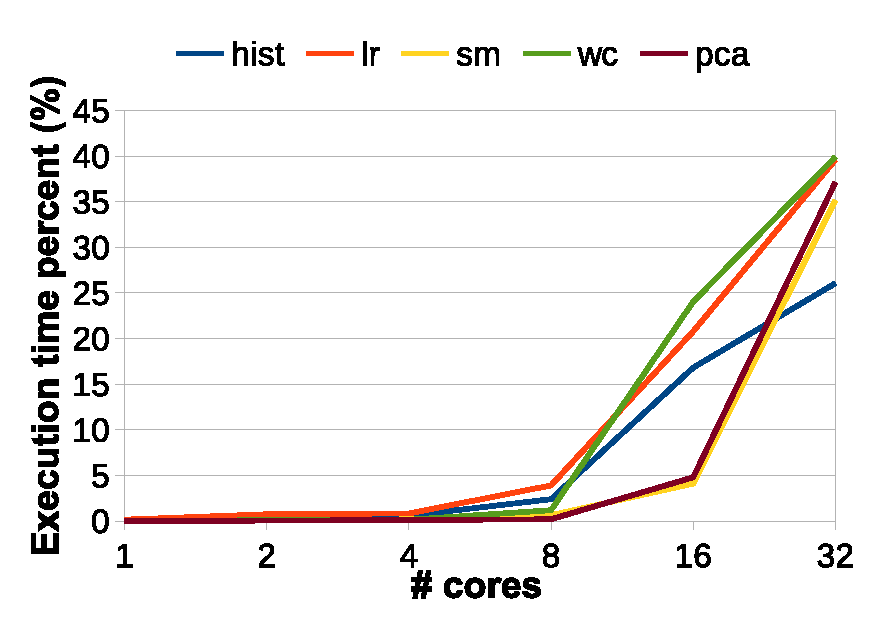
\includegraphics[width=0.45\textwidth]{eps/phoenix_spinlock_jemalloc.eps}
%	\caption{speedup of Phoenix-jemalloc}
%	\label{fig:phoenix:spinlock:jemalloc}
%\end{figure}
%The above performance changes can be explained from contending on the shared address space in Linux kernel.
%Therefore, we collect \_\_ticket\_spin\_lock execution time percent information to peek the contention by Linux perf.
%The results as shown in Figure \ref{fig:phoenix:spinlock:jemalloc}, turn out that serious lock contention takes place when increase the number of cores over 8 and as a result execution time will be drastically increased.
%
%
%%When the number of dependent processes increases above the
%%number of cores, serious contending lock takes place,
%%and as a result execution time will be drastically increased.
%%As the number of threads increases from 32 to 33, 
%%there is a significant increase in execution time owing to .
%
%Overall, increasing cores number results in the growth of speedup for Phoenix at low cores.
%However, as more cores were added, the benefit was reversed due to the increased time spent in spinlock.
%The results indicate that in spite of using the scalable memory allocator, Phoenix can not scale up to 16 cores.
%====================================================

%\subsection{Performance and Scalability}
%描述benchmarks的特点,benchmarks的数据集等


\subsubsection{Performance of SMR}
Based on \myth, we implemented the optimization of Phoenix in Section \ref{sec:runtime} and measured \myds performance by executing each benchmark. 
We compare the execution time of \myds with \codet{Phoenix-ptmalloc} and \codet{Phoenix-jemalloc}, respectively.
%\redt{Why use these benchmark?}
%Table II describes the workloads and their input datasets. 
\begin{figure}[!h!t]  
	\centering
	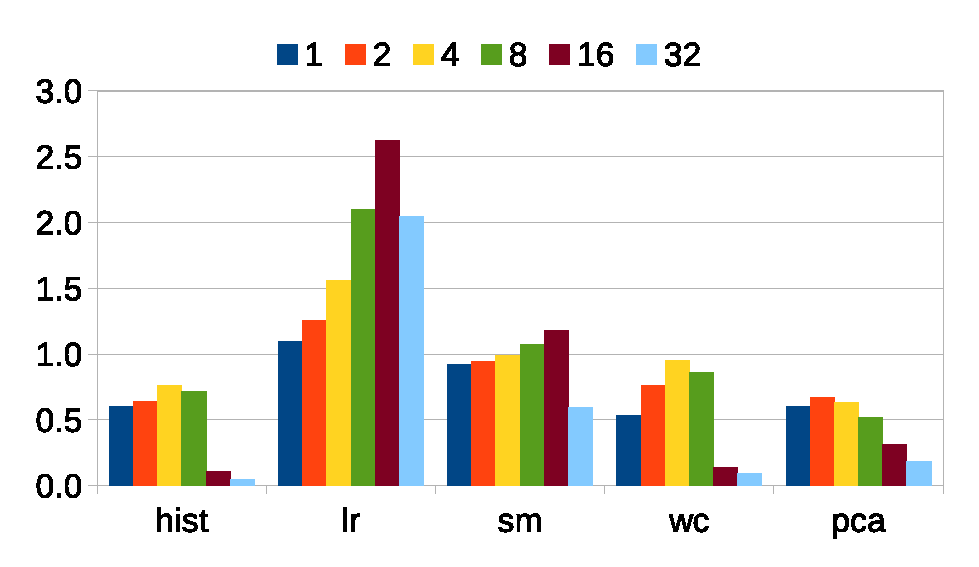
\includegraphics[width=0.45\textwidth]{eps/dmr_time_array.eps}
	\caption{SMR versus Phoenix with ptmalloc}
	\label{fig:smr:time:ptmalloc}
\end{figure}


%Firstly, we compare the execution time of \myds with \code{Phoenix-ptmalloc}.
Figure \ref{fig:smr:time:ptmalloc} shows the performance comparison between \myds and Phoenix2.
For \codet{hist}, \codet{wc} and \codet{pca}, the optimized runtime of \myds leads to improvement across all core counts.
The average improvement was \redt{2.0x} for less then 8 cores.
For more then 8 cores, specially with 16 and 32 cores, the improvement were obvious, reaching \redt{10.x} in maximum and \redt{5.0x} on average.
%and the variation across applications were rather small.
For \codet{sm}, it has performed as well as Phoenix when the cores number less then 16, while it surpasses Phoenix when there is more cores.
The only workload that \myds runs worse than Phoenix is \codet{lr}.
\begin{figure}[!h!t]  
	\centering
	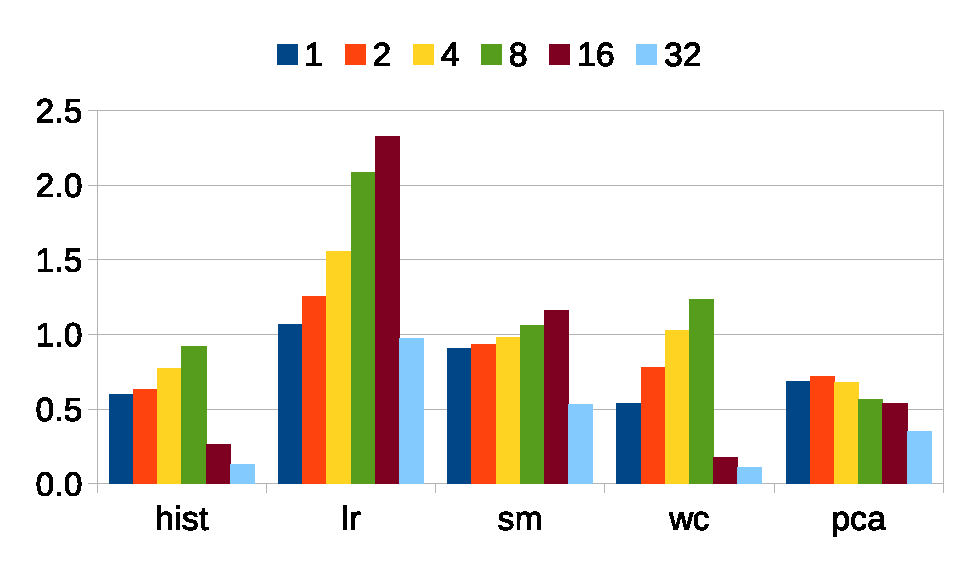
\includegraphics[width=0.45\textwidth]{eps/dmr_time_jemalloc.eps}
	\caption{SMR versus Phoenix with jemalloc}
	\label{fig:smr:time:jemalloc}
\end{figure}
Figure \ref{fig:smr:time:jemalloc} compares the performance of \myds against Phoenix built with jemalloc. 
%Figure 3 compares the performance of Phoenix++ against Phoenix 2

%Then, we compare the execution time of \myds with \codet{Phoenix-jemalloc}.
It can be saw that \codet{Phoenix-jemalloc} has a better performance, while the similar tendency like Figure \ref{fig:smr:time:ptmalloc}.
%when compare it with \myds, as showen in Figure \ref{fig:smr:time:jemalloc}, 
%we observe the similar tendency like Phoenix-ptmalloc.
%Then we observe the similar tendency when compare \myds with Phoenix-jemalloc in Figure \ref{fig:smr:time:jemalloc}, while Phoenix with jemalloc has a better performacne.


%Compared to Phoenix, we significantly increase the performance.
%Compared to Phoenix, 
The results indicate, for workloads, such as \codet{hist}, \codet{wc} and \codet{pca}, \myds performs significantly better than Phoenix, reducing the average running time to \redt{30\%}.
%the desired performance of \myds 
It owns to reducing the overhead caused by contending on the shared address space (Section \ref{sec:design}) and pipelining the Map and Reduce phase (Section \ref{sec:runtime}).
%However, workloads, such as \codet{lr} and \codet{sm}, still did not scale particularly well. 
However, \myds can not overcome Phoenix when running \codet{lr} and \codet{sm}. 
The reason of worse performance on \codet{lr} is that most of execution time is waste in \myds's initialization.
And for \codet{sm}, since it is a computation intensive workload, which does not cause many pagefault, Phoenix can scale well for these benchmarks in less cores.
We will evaluation overhead of initialization time in Section 5.4 and the bottlenecks of \myds will be discussed in detail in Section 5.4. 
%but in the remainder of this section we first focus on the optimizations that turned out to be successful.

%\redt{need to explain why hist, wc, pca has good performance,
	%实验的结果显示,lr在16核以上,spinlock的开销变大,而SMR的lr通过使用\myth避免这个问题,在16以下,从而获得较好的性能。lr较差的性能,是因为,相对Phoenix的版本,smr版本中用于初始化的花费的开销较大,导致其最终比Phoenix的版本的性能差(将会在5.4说明)hist,wc,pca, 具有较好的性能是,smr使用sthread避免spinlock的开销,同时将map和reduce进行pipeline,从而具有较好的性能。
%	 It is contrasted with 
%}

%\begin{figure}[htpb]
%	\centering
%	\subfigure[SMR versus Phoenix with ptmalloc]{
%		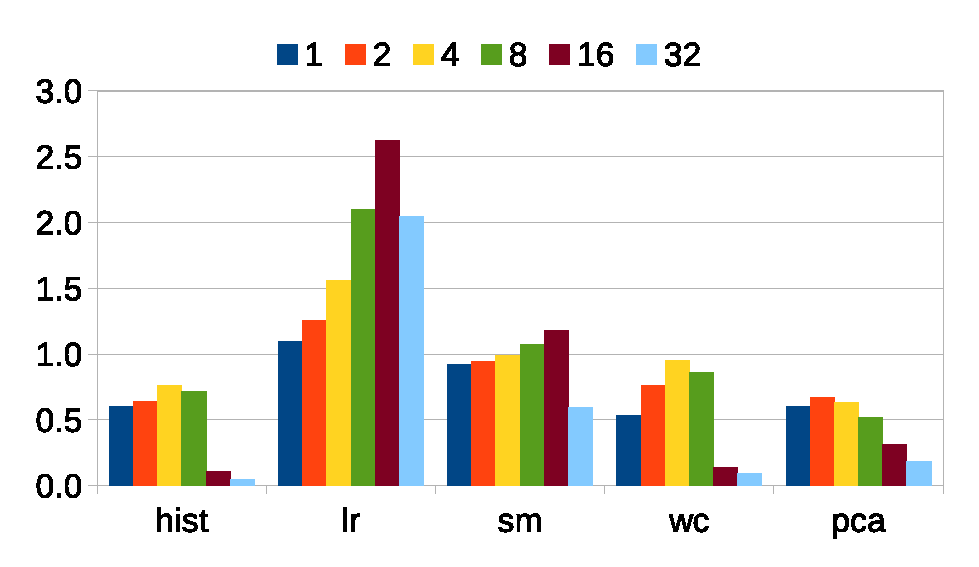
\includegraphics[width=0.45\textwidth]{eps/dmr_time_array.eps}
%		\label{fig:smr:time:ptmalloc}
%	}
%	\subfigure[SMR versus Phoenix with jemalloc]{
%		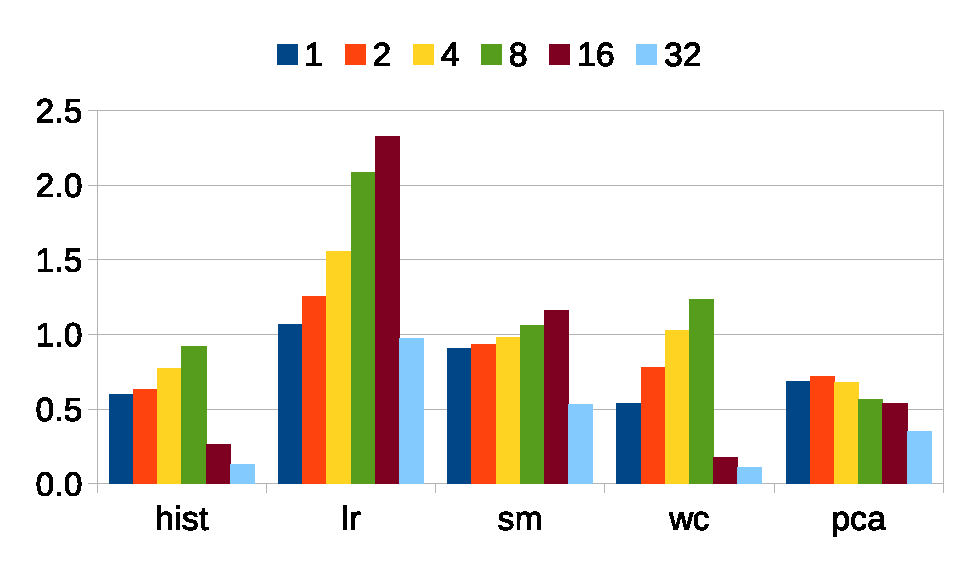
\includegraphics[width=0.45\textwidth]{eps/dmr_time_jemalloc.eps}
%		\label{fig:smr:time:jemalloc}
%	}
%	\caption{Execution time of SMR versus Phoenix}
%	\label{fig:time}
%\end{figure}


%However, nether allocator could successfully scaled up to 32cores.
%
%Figure\ref{fig:dmr:time:ptmalloc} and \ref{fig:dmr:time:jemalloc}
%present the Execution time of \myds versus Phoenix.
%%虽然jemalloc的性能表现要比ptmalloc好,但实验结果都显示
%\myds matches or outperforms Phoenix on 4 out of 5 workloads,
%but runs worse than Phoenix only on linear\_regression.
%For hist, pca and word\_count, 
%\myds outperforms Phoenix betwen xxx and xxx faster.

%从实验的结果可以看出,hist, wc, pca,SMR的性能较好,sm相当,lr中SMR的性能表现较差



%\begin{figure*}[htpb]
%\centering
%  \subfigure[]{
%   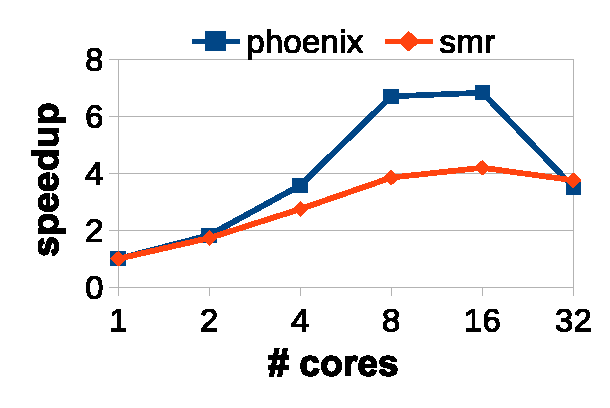
\includegraphics[width=0.15\textwidth]{eps/smr_scala_hist.eps}
%   \label{fig:dmr:time:ptmalloc}
%   }
%  \subfigure[]{
%	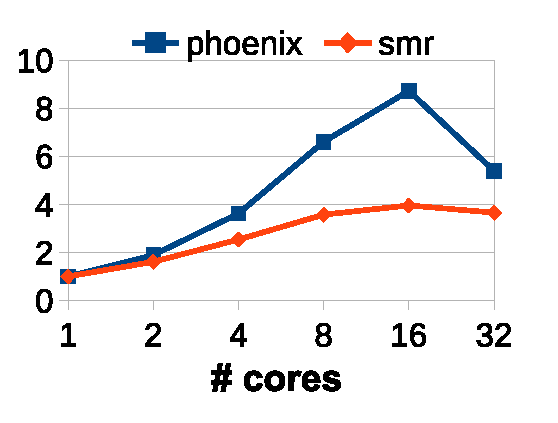
\includegraphics[width=0.15\textwidth]{eps/smr_scala_lr.eps}
%	\label{fig:dmr:time:ptmalloc}
%}
%  \subfigure[]{
%	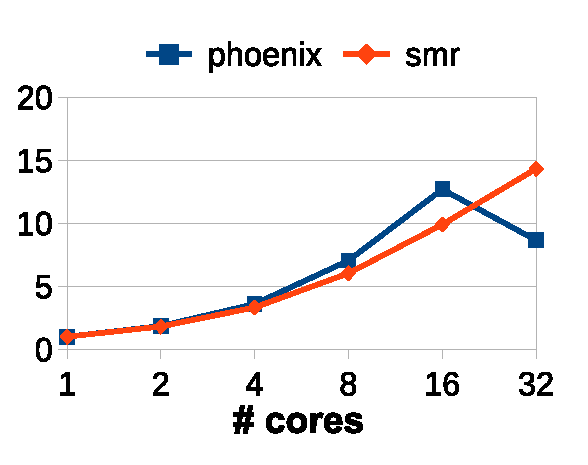
\includegraphics[width=0.15\textwidth]{eps/smr_scala_sm.eps}
%	\label{fig:dmr:time:ptmalloc}
%}
%  \subfigure[]{
%	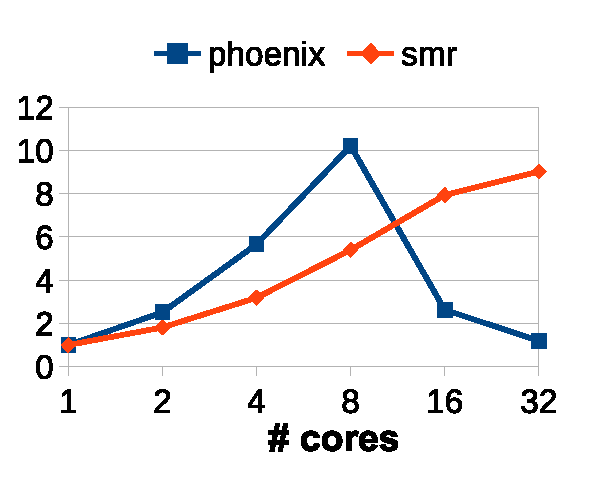
\includegraphics[width=0.15\textwidth]{eps/smr_scala_wc.eps}
%	\label{fig:dmr:time:ptmalloc}
%}
%  \subfigure[]{
%	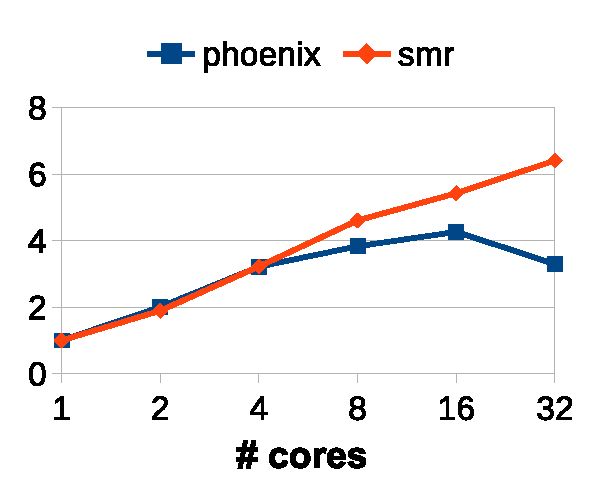
\includegraphics[width=0.15\textwidth]{eps/smr_scala_pca.eps}
%	\label{fig:dmr:time:ptmalloc}
%}
%  \caption{A comparison of the scalability of \myds with that of Phoenix}
%   \label{fig:scalability}
%\end{figure*}

\subsubsection{Scalability of SMR}
System Contention is evaluated using the execution time percent of \_\_ticket\_spin\_lock.
Figure \ref{fig:smr:spinlock} reports of \_\_ticket\_spin\_lock overhead in \myds.
Evaluation indicates that the lock overhead can be significantly reduced to less than 1\% of total runtime from 1 to 32 cores.
This demonstrates that using isolated-memory \myth thread can  
significantly reduce the contention in Linux kernel.
%\begin{figure}[htpb]
%	\centering
%	\subfigure[speedup of \myds]{
%		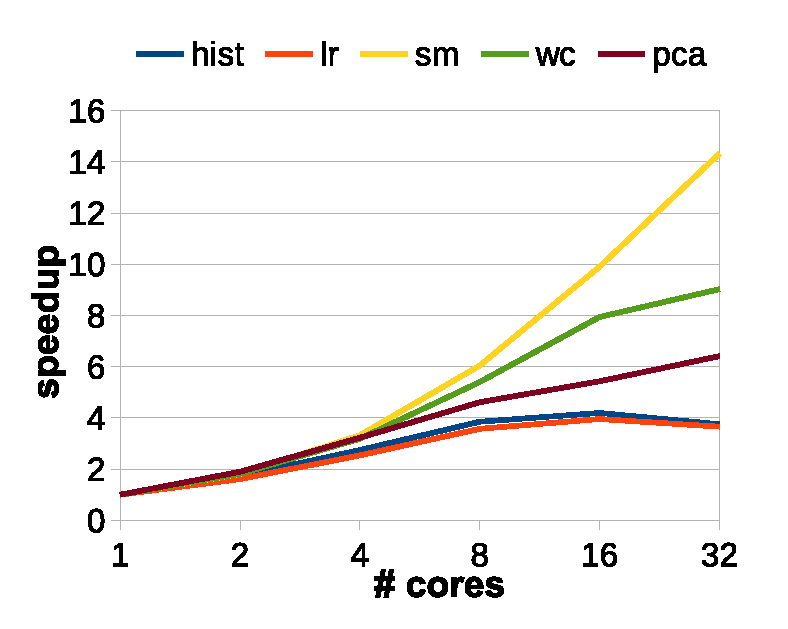
\includegraphics[width=0.45\textwidth]{eps/dmr_speedup.eps}
%		\label{fig:smr:speedup}
%	}
%	\subfigure[Execution time percent of \_\_tickect\_spin\_lock in \myds]{
%		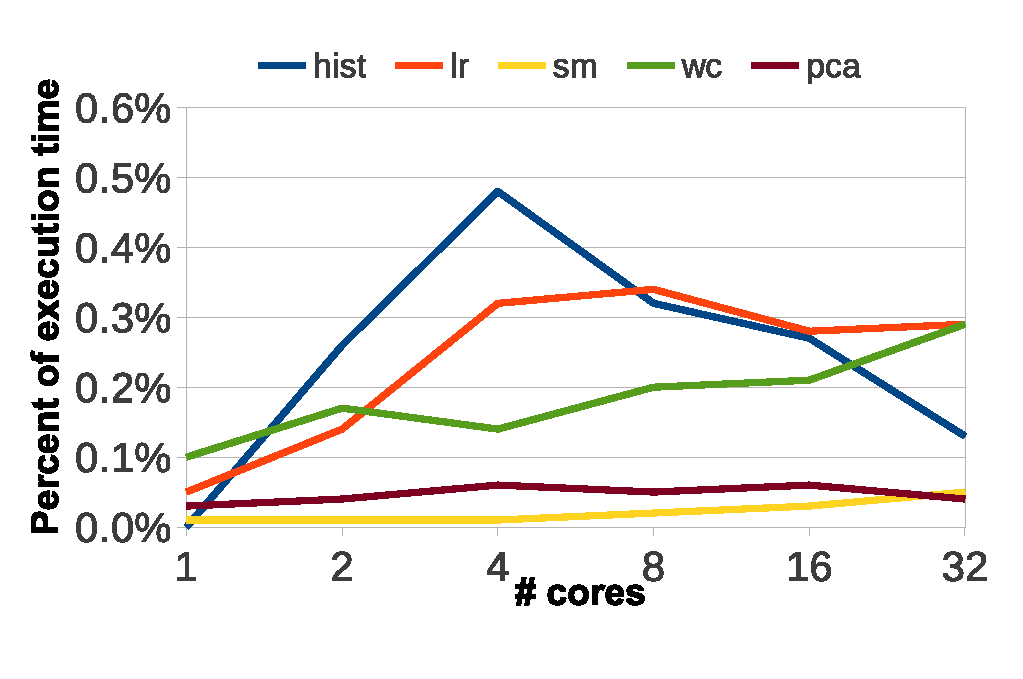
\includegraphics[width=0.45\textwidth]{eps/dmr_spinlock.eps}
%		\label{fig:smr:spinlock}
%	}
%	\caption{scalability of \myds}
%	\label{fig:smr:scalability}
%\end{figure}


 
\begin{figure}[!h!t]  
	\centering
	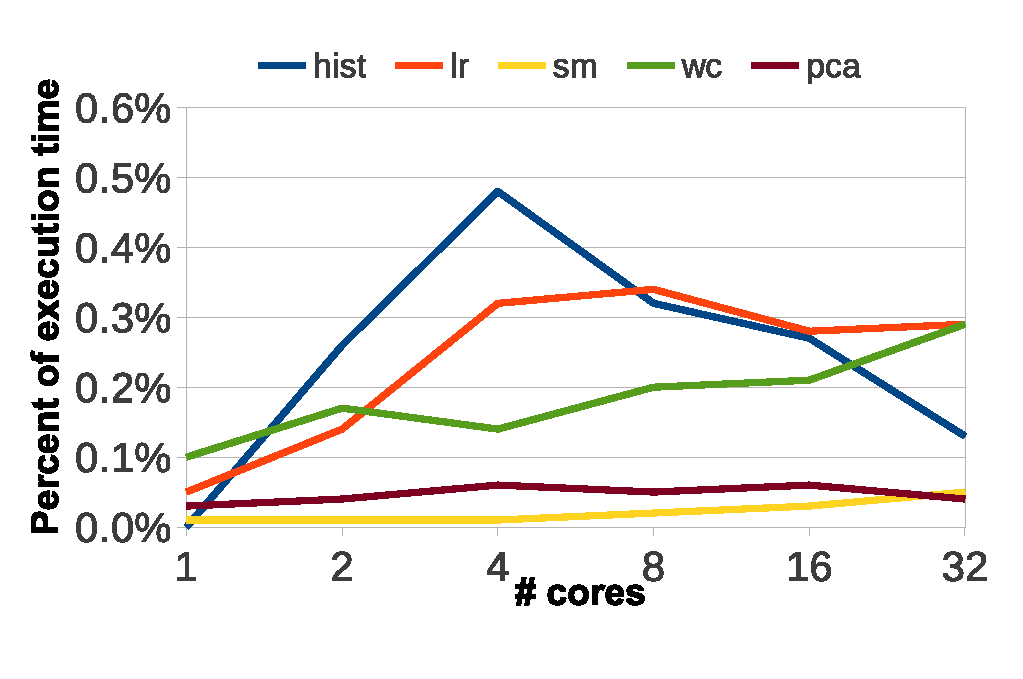
\includegraphics[width=0.45\textwidth]{eps/dmr_spinlock.eps}
	\caption{Execution time percent of \_\_tickect\_spin\_lock in \myds}
	\label{fig:smr:spinlock}
\end{figure}

 


\begin{figure}[!h!t]  
	\centering
	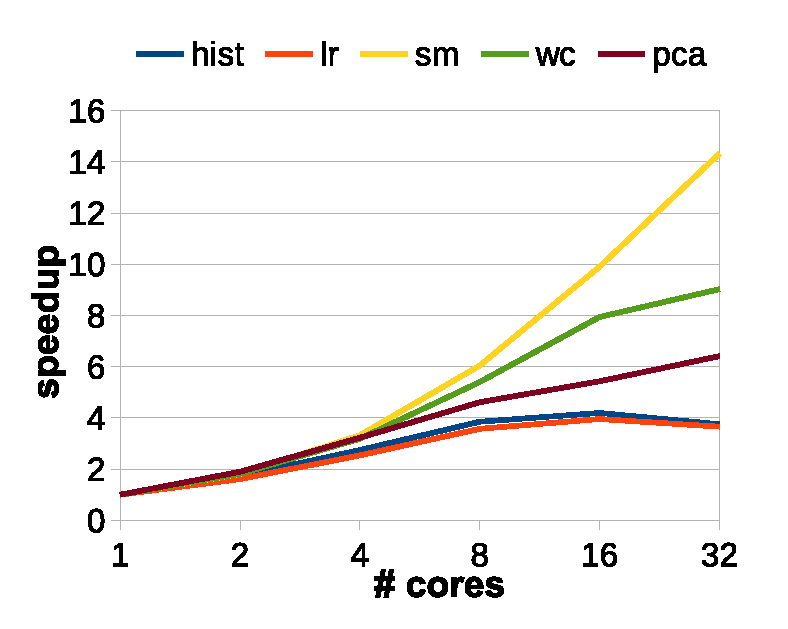
\includegraphics[width=0.45\textwidth]{eps/dmr_speedup.eps}
	\caption{speedup of \myds}
	\label{fig:smr:speedup}
\end{figure}
Figure \ref{fig:smr:speedup} summarizes the scalability results for \myds.
Specially, workloads \codet{sm}, \codet{wc} and \codet{pca} scale up to 32 cores.
And the performance of these applications is scale linearly with the number of cores.
However, \codet{linear\_regression} and \codet{histgram} still did not scale particularly because of wasting considerable time in initialization.
We will discuss this bottleneck in detail in subsection 5.4.



%\begin{figure}[!h!t]  
%	\centering
%	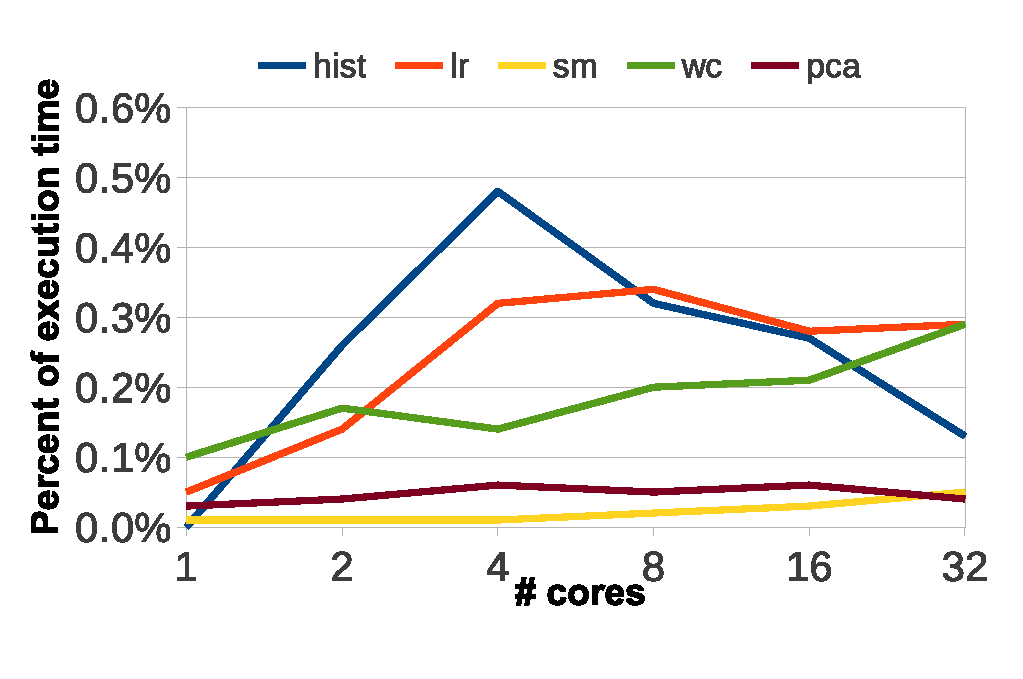
\includegraphics[width=0.45\textwidth]{eps/dmr_spinlock.eps}
%	\caption{tickect\_spin\_lock execution time percent of Phoenix}
%	\label{fig:smr:spinlock}
%\end{figure}

%We say a waiting thread is the thread which is waiting for shared
%data that produced by another thread. If using semaphore for
%synchronization, a waiting thread will be blocked and enlisted
%on the waiting queue by the OS scheduler. If using spinlock
%for synchronization, a waiting thread will do busy wait, i.e.
%spinning in a while loop. Embedded software applications
%that using semaphore to handle the synchronization could
%result in performance overkill, since it involves system calls
%translated into thousands of CPU instructions [1]; while using
%spinlock have problem of long busy-waiting time.

%When a running thread tries to read shared data,
%it must do busy wait until it has exhausted its time-slice
%or until another thread has withdrawn the occupation on the
%shared data. 




%System performance is evaluated using
%instructions per cycle (IPC). Higher IPC means
%better performance.
%Figure\ref{fig:perf:ipc} shows the IPC of Phoenix first increases 
%and then decreases as more threads are run on multi-core system.


Overall, for applications such as \codet{word\_count}, \codet{histgram} and \codet{pca}, the results show clearly that \myds has better performance and scalability when compared to Phoenix.
\myds has the advantage over Phoenix for pipelining map and reduce phases and separating address space by using \myth thread. 
However, for applications such as \codet{linear\_regression}, \myds does not show its superiority, which will be analyzed in detail in Section 5.4.

\subsection{Impact of buffer Optimizations}
In Section 4.3, we discussed the organization of intermediate data is critical to the performance of many MapReduce applications.
The default hash buffer need to gather the scatter key arrays together before sending them to the \codet{shared-channel}, which is time-wasting.
We addressed this issue by providing a array implementation of buffer, i.e., array buffer, which is a continuous memory space avoiding key value pairs coping and buffer reallocation.
%However, not all the workloads benefited from the optimization.

%As described in Section 4.3, we provide two implementation of the local buffer in Map phase, i.e, hash buffer or array buffer.  
\begin{figure}[!h!t]  
	\centering
	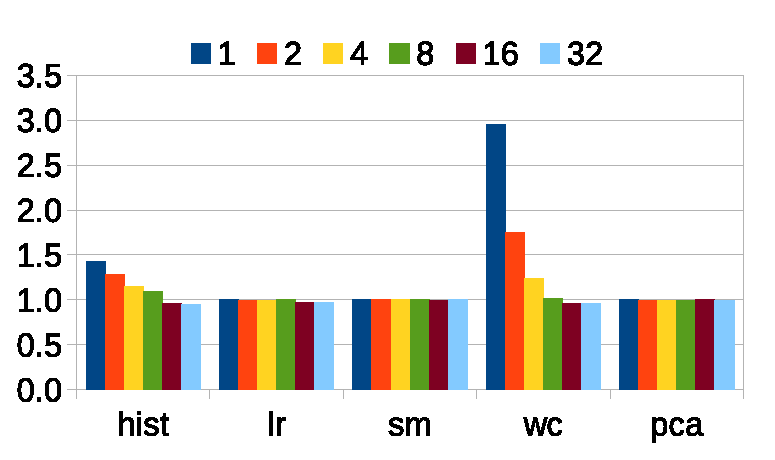
\includegraphics[width=0.45\textwidth]{eps/smr_diff_buffer.eps}
	\caption{Execution time of hash buffer over array buffer}
	\label{fig:smr:diff:buffer}
\end{figure}

%As the number of threads increases (from 1 to 8), the
%execution times for both Pthread/C and MPI programs decrease
%for both workstation and supercomputer. For 9 threads to 32
%threads, Pthread/C and MPI execution times changes slightly
%on workstation. However for 9 threads to 32 threads, both
%Pthread/C and MPI execution times keep decreasing (in most
%cases) with the increase in number of threads on the
%supercomputer node. This is because we use 8 cores in the
%workstation while we use 32 cores in the supercomputer node.
%Execution time for large number of threads (9 to 33 and
%beyond) remains almost the same for the workstation because
%of no communication overhead. Results (see Figure 4) also
%show that MPI execution time on supercomputer increases
%significantly when the number of threads is increased from 32
%to 33 and beyond; but Pthread/C execution time on
%supercomputer remains almost unchanged. This is due to the
%communication overhead among the cores (32 cores in a
%supercomputer node) when using MPI message passing.

To measure the impact of buffer's implementation for performance, we run all applications with hash buffer and array buffer, respectively.
Figure\ref{fig:smr:diff:buffer} compares the execution time of hash buffer and array buffer. 
From the Figure, it can be seen that although cases such as \codet{word\_count} and \codet{histgram} used array buffer has better performance, other benchmarks, e.g., \codet{linear\_regression}, \codet{string\_match} and \codet{pca}, did not.
A common feature of \codet{word\_count} and \codet{histgram} is that they will generate a large number of key-value pairs in MapReduce computation.
Therefore, gather operation waste more time in hash buffer, resulting in better performance by using array buffer.
%So, for workloads that generate a large number of key-value pairs, 

%From the experimental results, it is observed that benchmarks yield better performance using \myds than Phoenix (in most cases). 
%\myds has the advantage over Phoenix for pipelining map and reduce phases and separating address space by using \myth thread instead of shared memory Pthread. 
%The performance of the \codet{histgram} implementation on Phoenix is the best, 30\%-95\%x better than the Phoenix implementation on the our 32-cores system.

\subsection{ Challenges and Limitations}	
Although we were able to significantly improve the performance and scalability of \myds, 
workloads \codet{histogram} and \codet{linear\_regression} still did not scale up to 32cores (Figure \ref{fig:smr:speedup}).
In addition, \myds spent more time then Phoenix when run \codet{linear\_regression} (Figrure \ref{fig:smr:time:ptmalloc}). 
%Figure \ref{fig:smr:time:ptmalloc} presents their execution time at various core counts.
%We used /usr/bin/time to assess where the execution time was
To find out where the execution time was being spent, we collect each phase time information by using stub. 
The results denote that workloads on \myds waste more execution time in initialization phase when compared to Phoenix.

Figure \ref{fig:env:init}(a) and \ref{fig:env:init}(b) exhibit the initialization time of \myds and Phoenix, respectively.
The results show that the initialized time of \myds is range 0.25s to 0.35s, while it is just about 0.001s in Phoenix, which is far less than in \myds.
Moreover, except for \codet{pca}, we observe that initialized time is small variation for different benchmarks and in different cores count from Figure \ref{fig:env:init}(b).
Since there are two times mapreduce computation in \codet{pca}, which leads to two times initialization, it take more time than others benchmarks.
\begin{figure}[!h!t]  
	\centering
	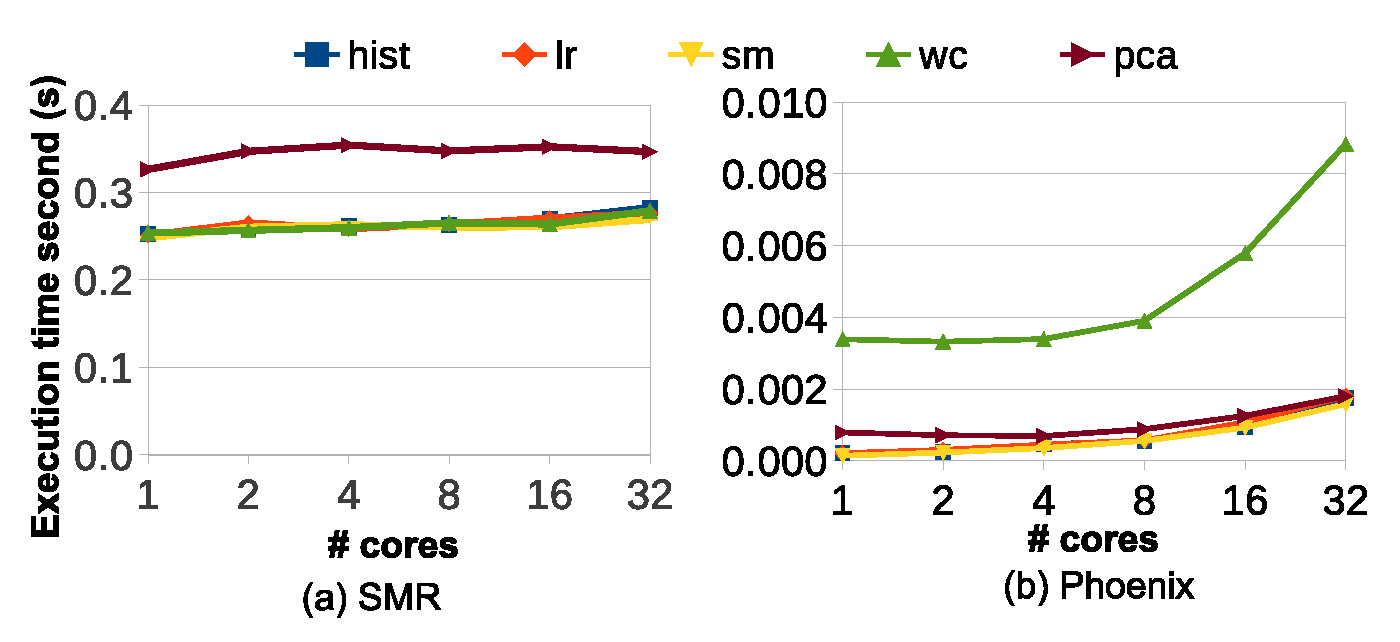
\includegraphics[width=0.5\textwidth]{eps/env_init.eps}
	\caption{initialization time of \myds and Phoenix}
	\label{fig:env:init}
\end{figure}


%解释为什么smr中的初始化时间会这么大
For multicore MapReduce workflow, most of initialized time is occupied in creating map and reduce threads.
Phoenix, in which multiple threads share the process's resource by using Pthread, can save time for creating threads.
On the contrary, there are many resource need to be allocated for each \myth thread, including separated address space, shared channel and setting up producer and consumer relationship.
As a result, \myds will take more time for in initialization.
%Compared to thread in Phoenix, which based on Pthread, creating thread will spend more time in \myds because of more resource need to be allocated.
%What's more, it will take more time for creating \codet{shared-channel} and setting up producer and consumer relationship for it in \myds.

  
\begin{figure}[htpb]
	\centering
	\subfigure[Execution time and initialization time on histgram]{
		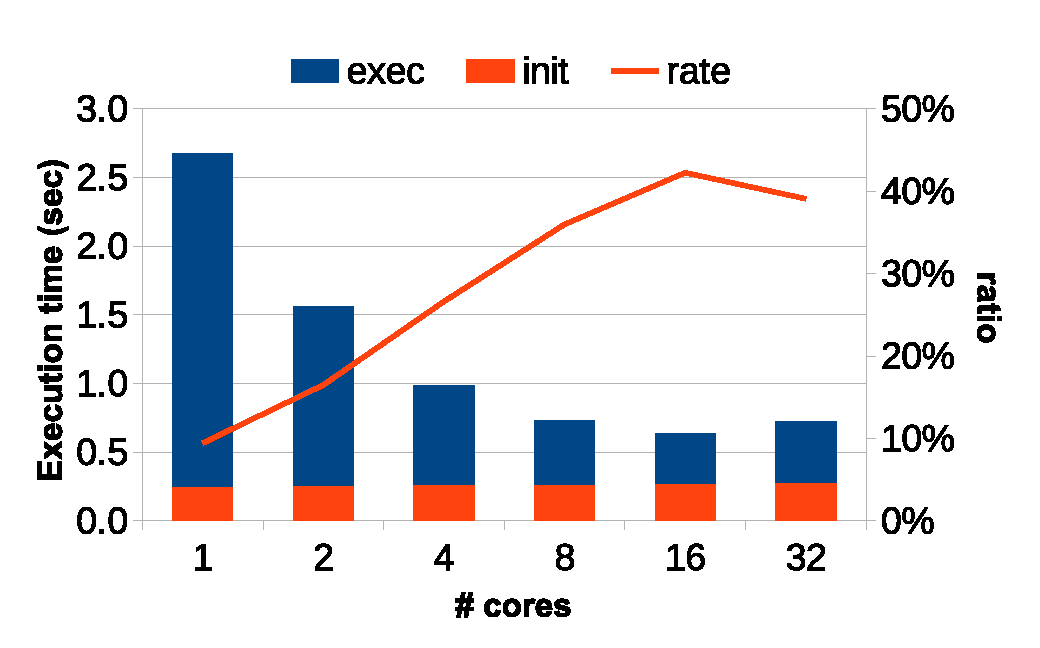
\includegraphics[width=0.45\textwidth]{eps/dmr_hist_init.eps}
		\label{fig:dmr:hist:init}
	}
	\subfigure[Execution time and initialization time on linear\_regression]{
		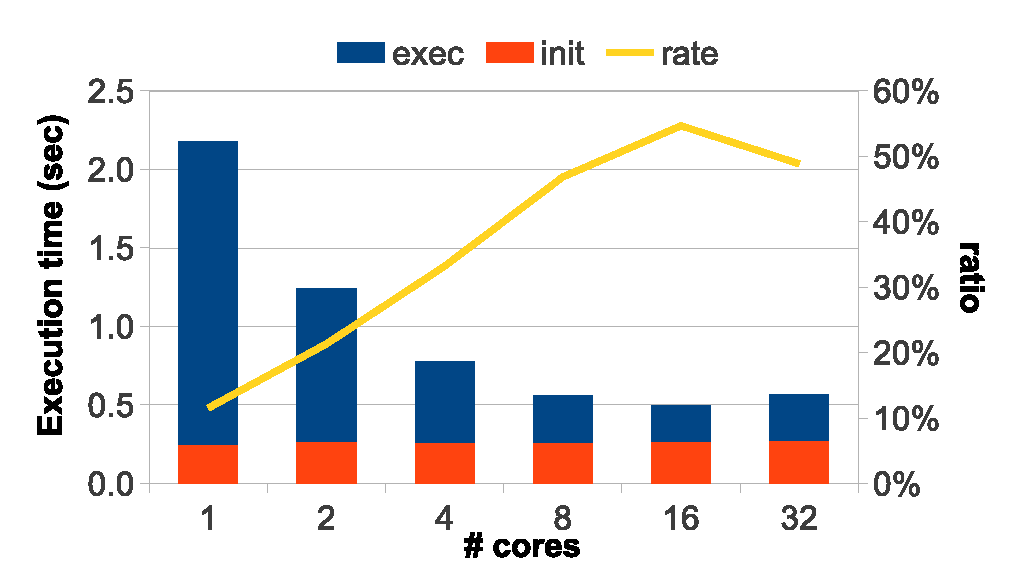
\includegraphics[width=0.45\textwidth]{eps/dmr_lr_init.eps}
		\label{fig:dmr:lr:init}
	}
	\caption{Initialize time with \myds}
	\label{fig:init}
\end{figure}


%这种较大较大的初始化对performance和scalability造成的影响


Figure \ref{fig:dmr:hist:init} shows the results with \codet{exec} defined as mapreduce actual execution time and \codet{init} as the initialization time. 
It was clear that the 2 non-scaling workloads (i.e., \codet{histgram} and \codet{linear\_regression}) share two common trends. 
First, the total execution time of both \codet{histgram} and \codet{linear\_regression} less than 2.7s for all cores, which is far less than other benchmarks. 
Second, as the increasing number of cores, the portion of actual computation time (i.e., \codet{exec}) significantly decreased.
However, the initialization time (i.e., \codet{init}) is almost constant, which cause the \codet{init} time ratio increase and dominate the total execution time at high cores count. 
As a result,  \codet{histgram} and \codet{linear\_regression} can not scale up to 32 cores.
And the total execution time of \codet{linear\_regression} on Phoenix will less than on \myds.
%Second, the portion of actual computation time assumed by kernel code (sys /
%effective) significantly increased as we went beyond the single
%chip boundary.
%Second, both total execution time are short, While the portion of init time is 





